% 
% (c) Copyright 2016 Tabea Mendez
% 
% This source is free: you can redistribute it and/or modify
% it under the terms of the GNU General Public License as published by
% the Free Software Foundation, either version 3 of the License, or
% (at your option) any later version.
% 
% This source is distributed in the hope that it will be useful,
% but WITHOUT ANY WARRANTY; without even the implied warranty of
% MERCHANTABILITY or FITNESS FOR A PARTICULAR PURPOSE.  See the
% GNU General Public License for more details.
% 
% You should have received a copy of the GNU General Public License
% along with this source.  If not, see <http://www.gnu.org/licenses/>.
%
%%%%%%%%%%%%%%%%%%%%%%%%%%%%%%%%%%%%%%%%%%%%%%%%%%%%%%%%%%%%%%%%%%%%%%%%%%%%%%

\section{Rausch-Reduktions-Filter}
	\begin{goal}
	 \begin{minipage}{0.8\textwidth}
	 $ $\\Das Ziel eines Rausch-Reduktions-Filters $H(z)$ ist es, das eigentliche Signal $x_S(n)$ aus dem Messsignal $x(n)$ herauszufiltern und dabei das Rauschen $x_V(n)$ zu unterdrücken.\\
	 $\;\begin{array}{l}\text{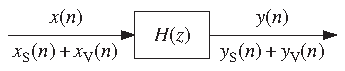
\includegraphics[width = 0.45\textwidth]{pic/NoiseRedFilterTime.pdf}}\end{array}\qquad$\fcolorbox{CadetRed}{white}{$\begin{array}{lcl}y_S(n) &= &x_S(n-delay)\\y_V(n) &=& 0\end{array}$}
	 \end{minipage}
	\end{goal}\\[-0.3cm]

	\subsection{Ideales Rausch-Reduktions-Filter}
		Damit das Rauschen vollkommen unterdrückt werden kann ohne das eigentliche Signal $x_S(n)$ zu verändern muss im Frequenzbereich folgendes gelten:\\
		\begin{minipage}{0.36\textwidth}
			\fcolorbox{CadetRed}{white}{$\begin{array}{l}Y_S(\omega)\; =\; H(\omega)\,X_S(\omega)\; =\; X_S(\omega)\\Y_V(\omega)\, = \;H(\omega)\,X_V(\omega) \,= \;0\end{array}$}\\[0.2cm]
			$\begin{array}{ll}\Rightarrow&\;\textbf{Die beiden Spektren $X_S(\omega)$}\\&\;\textbf{und $X_V(\omega)$ dürfen nicht}\\&\;\textbf{überlappen!}\end{array}$\\[0.2cm]
		\end{minipage}
		\begin{minipage}{0.67\textwidth}
		 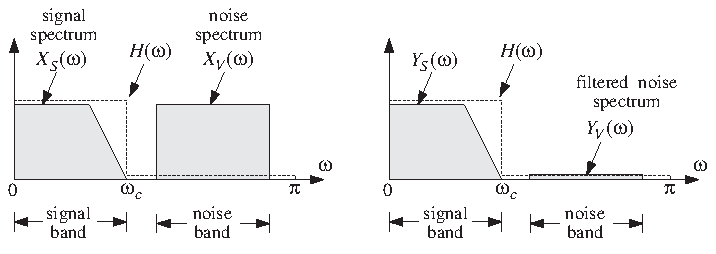
\includegraphics[width = \textwidth]{pic/NoiseRedFilterIdeal.pdf}
		\end{minipage}

	\subsection{Bestmögliches Rausch-Reduktions-Filter}
		Ist das ideale Rausch-Reduktions-Filter nicht realisierbar, weil die beiden Spektren $X_S(\omega)$ und $X_V(\omega)$ überlappen ist die bestmögliche Lösung ein \textbf{idealer Bandpass} (hier Tiefpass).\\[-0.5cm]
		\begin{itemize}
			 \item Das eigentliches Signal $x_S(n)$ wird nicht verzerrt.$\qquad$
			 \fcolorbox{CadetRed}{white}{$Y_S(\omega)\; =\; H(\omega)\,X_S(\omega)\; =\; X_S(\omega)$}\\[-0.5cm]
			 \item Das Rauschen $x_V(n)$ wird maximal unterdrückt.\\[-0.5cm]
			\end{itemize}
		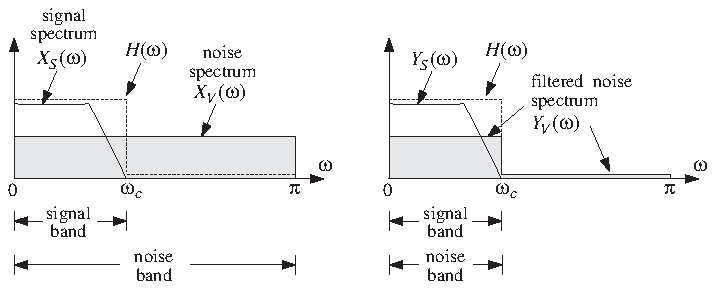
\includegraphics[width = 0.7\textwidth]{pic/NoiseRedFilter.pdf}\\[-0.1cm]
		\textbf{Rauschen:}\\[0.15cm]
		Für ein Mittelwertfreies-Weisses-Rauschen $x_V(n)$ gelten folgende Beziehungen:\\[0.2cm]
		\begin{tabular}{ll}
			Leistungsdichtespektrum und Leistung des&\multirow{2}{*}{\fcolorbox{CadetRed}{white}{$S_{X_VX_V}(\omega) = \sigma_{X_V}^2$}}\\
			Mittelwertfreiem-Weissem-Rauschen $x_V(n)$&\\[0.2cm]
			Leistungsdichtespektren des &\multirow{2}{*}{\fcolorbox{CadetRed}{white}{$S_{Y_VY_V}(\omega) =\big|H(\omega)\big|^2 \, S_{X_VX_V}(\omega)=\big|H(\omega)\big|^2 \, \sigma_{X_V}^2 $}}\\
			Farbigen-Ausgangsrauschen $y_V(n)$&\\[0.3cm]
			Leistung des Farbigen-Ausgangsrauschen&\fcolorbox{CadetRed}{white}{$\sigma_{Y_V}^2 = \dfrac{1}{2\pi}\myint{-\pi}{\pi}{S_{Y_VY_V}(\omega)}{\omega}= \sigma_{X_V}^2\dfrac{1}{2\pi}\myint{-\pi}{\pi}{\big|H(\omega)\big|^2}{\omega}= \sigma_{X_V}^2\,NRR$}\\[0.8cm]
			Noise-Reduction-Ratio NRR &\multirow{2}{*}{\fcolorbox{CadetRed}{white}{$NRR = \dfrac{\sigma_{Y_V}^2}{\sigma_{X_V}^2}= \dfrac{1}{2\pi}\myint{-\pi}{\pi}{\big|H(\omega)\big|^2}{\omega} = \mysum{n}{}{h(n)^2}$}}\\
			(sollte möglichst klein sein)&\\[0.3cm]
		\end{tabular}\\[0.2cm]
		\textbf{Signal-Rausch-Abstand SNR:}\\[0.2cm]
		Durch das Rausch-Reduktions-Filter ergeben sich folgende Signal-Rausch-Abstände:\\[0.2cm]
		\begin{tabular}{ll}
			SNR am Eingang & \fcolorbox{CadetRed}{white}{$\text{SNR}_{in} = \dfrac{E[x_S(n)^2]}{E[x_V(n)^2]} $}$\qquad\qquad\qquad$SNR am Ausgang $\quad$ \fcolorbox{CadetRed}{white}{$\text{SNR}_{out} = \dfrac{E[y_S(n)^2]}{E[y_V(n)^2]} $}\\[0.7cm]
			SNR-Verbesserung & \fcolorbox{CadetRed}{white}{$\dfrac{\text{SNR}_{out}}{\text{SNR}_{in}} = \dfrac{E[y_S(n)^2]}{E[y_V(n)^2]}\cdot \dfrac{E[x_V(n)^2]}{E[x_S(n)^2]}
			= \underbrace{\dfrac{E[x_V(n)^2]}{E[y_V(n)^2]}}_{1/NRR}\cdot \dfrac{E[y_S(n)^2]}{E[x_S(n)^2]}$}\\[1.3cm]
			&$\;\Rightarrow\quad$ Wenn das Signal $x_S(n)$ durch das Filter $H(\omega)$ nicht verändert wird gilt:\\[0.2cm]
			& $\qquad\quad$\fcolorbox{CadetRed}{white}{$\dfrac{\text{SNR}_{out}}{\text{SNR}_{in}} = \dfrac{1}{NRR}$}\\
		\end{tabular}\\[0.2cm]
		\textbf{NRR von idealen Filtern:}\\[0.2cm]
		\begin{tabular}{ll}
			Idealer Tiefpass & \fcolorbox{CadetRed}{white}{$NRR = \dfrac{\sigma_{Y_V}^2}{\sigma_{X_V}^2}= \dfrac{1}{2\pi}\myint{-\omega_c}{\omega_c}{1}{\omega} = \dfrac{2\omega_c}{2\pi} = \dfrac{\omega_c}{\pi}$}\\[0.8cm]
			Idealer Bandpass & \fcolorbox{CadetRed}{white}{$NRR = \dfrac{\sigma_{Y_V}^2}{\sigma_{X_V}^2}= \dfrac{2}{2\pi}\myint{\omega_a}{\omega_b}{1}{\omega} = \dfrac{\omega_b-\omega_a}{\pi}$}\\
		\end{tabular}\\[0.2cm]
	\subsection{Reale Rausch-Reduktions-Filter}
		Ideale Filter mit einer unendlich kurzen Übergangsbandbreite können nicht implementiert werden.\\
		Reale Rausch-Reduktions-Filter haben eine gewisse Übergangsbandbreite und sind oft linearphasig.\\[0.3cm]
		\begin{tabularx}{\textwidth}{|rp{4cm}p{9cm}X|}
		 \hline&&&\\[-0.3cm]
			\multicolumn{4}{|l|}{\textbf{IIR-Smoother erster Ordnung}}\\[-0.35cm]
			&&&
			\begin{tikzpicture}[>=latex, scale=1.2]
				\def\s{2.7};
				\def\f{1.15};
				\def\r{0.9};
				\def\roc{0.9};
				\coordinate (c1) at (0,0);
				\draw[line width=0.5](c1)++(-\s/2,-\s/2)node[above right]{ }--++(\s,0)--++(0,\s)node[below left]{\small$z$-Plane}--++(-\s,0)--cycle node[below right, CadetRed]{\textbf{ }};
				\draw[line width=0.75](c1)--++(-\f,0)--++(2*\f,0)--++(-\f,0)--++(0,-\f)--++(0,2*\f)--++(0,-\f)circle(0);
				\draw[line width=0.75,dashed](c1)circle(\roc);
				\draw[line width=0.75](c1)++(\roc,0.1)--++(0,-0.2)node[below right=-3pt,yshift=2pt]{$1$};
				\draw[line width=0.75](c1)++(-\roc,0.1)--++(0,-0.2)node[below left=-3pt,yshift=2pt]{\small-$1$};
				\draw[line width=0.75,fill,CadetRed](c1)++(0.65,0)circle(\r/15)node[below=2pt]{\small$a$};
% 				\draw[CadetRed,line width=0.75,fill=white](c1)++(0.75,-0.5)circle(\r/15)node[below left=-2pt]{$z_1$};

			\end{tikzpicture}\\[-2.85cm]
			$\;\,\bullet\!\!\!$ & \multicolumn{2}{p{13cm}}{Geeignet für DC-Signale $x_S(n)$}&\\[0.25cm]
			$\;\,\bullet\!\!\!$ & \multicolumn{2}{p{13cm}}{Mittelung über alle bisherigen Samples, wobei die Samples mit dem Faktor $a^d\,b\,x(n-d)$ gewichtet werden. Je weiter ein Sample zurückliegt, desto weniger } &\\
			&Einfluss hat es.&\fcolorbox{CadetRed}{white}{$y(n) = b\,x(n) + a\,y(n-1)$}$\qquad$\fcolorbox{black}{white}{$b = 1-a$}&\\[0.3cm]
			$\;\,\bullet\!\!\!$ &  Signalband:&\fcolorbox{black}{white}{$\omega = 0$}&\\[0.2cm]
			$\;\,\bullet\!\!\!$ & Übertragungsfunktion: &\fcolorbox{CadetRed}{white}{$H(z) = \dfrac{b}{1-a\,z^{-1}}\qquad\Rightarrow\qquad \big|H(\omega)\big|^2 =\dfrac{b^2}{1-2\,a\cos(\omega) + a^2}$}&\\[0.6cm]
			$\;\,\bullet\!\!\!$ & Grenzfrequenz: &\fcolorbox{CadetRed}{white}{$\big|H(\omega_c)\big|^2 = \dfrac{1}{2}\qquad\Rightarrow\qquad \cos(\omega_c) = 1-\dfrac{(1-a)^2}{2\,a}$}&\\[0.5cm]
			$\;\,\bullet\!\!\!$ & DC- und AC-Gain: &\fcolorbox{CadetRed}{white}{DC:$\;\;H(z)\big|_{z=1} = \dfrac{b}{1-a} = 1\qquad$AC:$\;\; H(z)\big|_{z=-1} = \dfrac{1-a}{1+a}$}&\\[0.5cm]
			$\;\,\bullet\!\!\!$ & Noise-Reduction-Ratio: &\fcolorbox{CadetRed}{white}{$NRR = \dfrac{1-a}{1+a}$}$\begin{array}{l}\text{$\qquad\quad\!$ Einschwingzeit:$\qquad$\fcolorbox{CadetRed}{white}{ $n_\text{eff} = \dfrac{\ln(\epsilon)}{\ln(a)}$}}\end{array}$&\\[0.6cm]
		\hline
		\end{tabularx}
		\begin{tabularx}{\textwidth}{|rp{4cm}p{9cm}X|}
		\hline&&&\\[-0.3cm]
			\multicolumn{4}{|l|}{\textbf{IIR-Smoother erster Ordnung mit bestimmter Grenzfrequenz}}\\[-0.35cm]
			&&&
			\begin{tikzpicture}[>=latex, scale=1.2]
				\def\s{2.7};
				\def\f{1.15};
				\def\r{0.9};
				\def\roc{0.9};
				\coordinate (c1) at (0,0);
				\draw[line width=0.5](c1)++(-\s/2,-\s/2)node[above right]{ }--++(\s,0)--++(0,\s)node[below left]{\small$z$-Plane}--++(-\s,0)--cycle node[below right, CadetRed]{\textbf{ }};
				\draw[line width=0.75](c1)--++(-\f,0)--++(2*\f,0)--++(-\f,0)--++(0,-\f)--++(0,2*\f)--++(0,-\f)circle(0);
				\draw[line width=0.75,dashed](c1)circle(\roc);
				\draw[line width=0.75](c1)++(\roc,0.1)--++(0,-0.2)node[below right=-3pt,yshift=2pt]{$1$};
				\draw[line width=0.75](c1)++(-\roc,0.1)--++(0,-0.2)node[below left=-3pt,yshift=2pt]{\small-$1$};
				\draw[line width=0.75,fill,CadetRed](c1)++(0.65,0)circle(\r/15)node[below=2pt]{\small$a$};
				\draw[CadetRed,line width=0.75,fill=white](c1)++(-0.9,0)circle(\r/15);%node[below left=-2pt]{$z_1$};

			\end{tikzpicture}\\[-2.85cm]
			$\;\,\bullet\!\!\!$ & \multicolumn{2}{p{13cm}}{Geeignet für DC-Signale $x_S(n)$}&\\[0.25cm]
			$\;\,\bullet\!\!\!$ & \multicolumn{2}{p{13cm}}{Mittelung über alle bisherigen Samples, wobei die Samples mit dem Faktor $(a^d+a^{d-1})\,b\,x(n-d)$ gewichtet werden. Je weiter ein Sample zurückliegt, desto} &\\
			&weniger Einfluss hat es.&\fcolorbox{CadetRed}{white}{$y(n) = b\,x(n) +b\,x(n-1) + a\,y(n-1)$}&\\[0.2cm]
			&&\fcolorbox{black}{white}{$a = \dfrac{1-\tan(\omega_c/2)}{1+\tan(\omega_c/2)}$}$\qquad$\fcolorbox{black}{white}{$b = \dfrac{1-a}{2}$}&\\[0.6cm]
			$\;\,\bullet\!\!\!$ &  Signalband:&\fcolorbox{black}{white}{$\omega = 0$}&\\[0.25cm]
			$\;\,\bullet\!\!\!$ & Übertragungsfunktion: &\fcolorbox{CadetRed}{white}{$H(z) = \dfrac{b\,(1+z^{-1})}{1-a\,z^{-1}}\qquad\Rightarrow\qquad \big|H(\omega)\big|^2 =\dfrac{2b^2(1+\cos(\omega))}{1-2\,a\cos(\omega) + a^2}$}&\\[0.6cm]
			$\;\,\bullet\!\!\!$ & Grenzfrequenz: &\fcolorbox{CadetRed}{white}{$\big|H(\omega_c)\big|^2 = \dfrac{1}{2}\qquad\Rightarrow\qquad \cos(\omega_c) = \dfrac{2\,a}{1+a^2}$}&\\[0.5cm]
			$\;\,\bullet\!\!\!$ & DC- und AC-Gain: &\fcolorbox{CadetRed}{white}{DC:$\;\;H(z)\big|_{z=1} = \dfrac{2b}{1-a} = 1\qquad$AC:$\;\; H(z)\big|_{z=-1} = 0$}&\\[0.5cm]
			$\;\,\bullet\!\!\!$ & Noise-Reduction-Ratio: &\fcolorbox{CadetRed}{white}{$NRR = \dfrac{1-a}{2}$}$\begin{array}{l}\text{$\qquad\quad\!$ Einschwingzeit:$\qquad$\fcolorbox{CadetRed}{white}{ $n_\text{eff} = \dfrac{\ln(\epsilon)}{\ln(a)}$}}\end{array}$&\\[0.6cm]
		 \hline&&&\\[-0.3cm]
			\multicolumn{4}{|l|}{\textbf{FIR-Mittelungs-Filter}}\\[-0.35cm]
			&&&
			\hspace*{-0.2cm}\begin{tikzpicture}[>=latex, scale=1.2]
				\def\s{2.7};
				\def\f{1.15};
				\def\r{0.9};
				\def\roc{0.9};
				\def\n{11};
				\coordinate (c1) at (0,0);
				\draw[line width=0.5](c1)++(-\s/2,-\s/2)node[above right,yshift=-3pt]{\footnotesize $k=1,2,...,N-1$}--++(\s,0)--++(0,\s)node[below left]{\small$z$-Plane}--++(-\s,0)--cycle node[below right, CadetRed]{\textbf{ }};
				\draw[line width=0.75](c1)--++(-\f,0)--++(2*\f,0)--++(-\f,0)--++(0,-\f)--++(0,2*\f)--++(0,-\f)circle(0);
				\draw[line width=0.75,dashed](c1)circle(\roc);
				\draw[line width=0.75](c1)++(\roc,0.1)--++(0,-0.2)node[below right=-3pt,yshift=2pt]{$1$};
				\draw[line width=0.75](c1)++(-\roc,0.1)--++(0,-0.2)node[below left=-3pt,yshift=2pt]{-$1$};

				\draw[line width=2,white](c1)++(\s/2,0)--++(0,0.65);

				\draw[line width=0.75,dotted](c1)--++({360*0/\n}:1.2);
				\draw[line width=0.75,->](c1)++({360*0/\n}:1.05)arc({360*0/\n}:{360*1/\n}:1.05)node[below right, xshift=3pt,yshift=5pt]{\Large$\frac{2\pi k}{N}$};
				\draw[line width=0.75,dotted](c1)--++({360*1/\n}:1.2);



% 				\draw[line width=0.75,fill,CadetRed](c1)++(0.65,0)circle(\r/15)node[below=2pt]{\small$a$};
				\foreach \i in {1,2,...,10}
				{
					\draw[CadetRed,line width=0.75,fill=white](c1)++({360*\i/\n}:0.9)circle(\r/15);
				}
			\end{tikzpicture}\\[-2.85cm]
			$\;\,\bullet\!\!\!$ & \multicolumn{2}{p{13cm}}{Geeignet für DC-Signale und tieffrequente Signale $x_S(n)$}&\\[0.25cm]
			$\;\,\bullet\!\!\!$ & \multicolumn{2}{p{13cm}}{Mittelung über die letzten $N$ Samples, wobei alle gleich stark gewichtet werden ($1/N$), da dadurch die $NNR$ minimiert wird.} &\\[0.6cm]
			&\multicolumn{2}{p{13cm}}{\fcolorbox{CadetRed}{white}{$y(n) = \dfrac{1}{N}\big(x(n)+x(n-1)+x(n-2)+...+x(n-(N-1))\big)$}}&\\[0.5cm]
			$\;\,\bullet\!\!\!$ &  Signalband:&\fcolorbox{black}{white}{$0\leq\omega\leq\omega_c$}&\\[0.25cm]
			$\;\,\bullet\!\!\!$ & Übertragungsfunktion: &\fcolorbox{CadetRed}{white}{$H(z) = \dfrac{1}{N}\big(1+z^{-1}+...+z^{-(N-1)}\big)=\dfrac{1}{N}\,\dfrac{1-z^{-N}}{1-z^{-1}}$}&\\[0.6cm]
			$\;\,\bullet\!\!\!$ & Frequenzgang: &\fcolorbox{CadetRed}{white}{$\big|H(\omega)\big|^2 =\dfrac{1}{N^2}\,\dfrac{\sin^2(N\omega/2)}{\sin^2(\omega/2)}$}&\\[0.6cm]
			$\;\,\bullet\!\!\!$ & Grenzfrequenz: &\fcolorbox{CadetRed}{white}{$\big|H(\omega_c)\big|^2 \;\stackrel{\mathrm{N \text{ gross}}}\approx\; \dfrac{4}{\pi^2}\approx 0.41\;\;\widehat=\;\; 3.9\db\qquad\Rightarrow\qquad \omega_c = \dfrac{\pi}{N}$}&\\[0.5cm]
			$\;\,\bullet\!\!\!$ & DC- und AC-Gain: &\fcolorbox{CadetRed}{white}{DC:$\;\;H(z)\big|_{z=1}  = 1\qquad$AC:$\;\; H(z)\big|_{z=-1} =\small\begin{cases} 0,& N\text{ gerade}\\ 1/N,& N\text{ ungerade}\end{cases}$}&\\[0.6cm]
			$\;\,\bullet\!\!\!$ & Noise-Reduction-Ratio: &\fcolorbox{CadetRed}{white}{$NRR = \dfrac{1}{N}$}$\begin{array}{l}\text{$\qquad\quad\!$ Einschwingzeit:$\qquad$\fcolorbox{CadetRed}{white}{ $n_\text{eff} = N$}}\end{array}$&\\[0.5cm]
		 \hline
		\end{tabularx}
\newpage
			
\section{Notch- und Comb-Filter}
	Diese Filter sind gut geeignet, wenn das Rauchen $x_V(n)$ oder das Signal $x_S(N)$ periodisch sind.\\[-0.6cm]
	\begin{itemize}
	 \item \textbf{Notch-Filter:} Das periodische Rauschen (50 Hz Netzbrummen) wird durch Notches (Kerben) bei den Rauschfrequenzen vernichtet.\\[-0.6cm]
	 \item \textbf{Comb-Filter:} Die Spektrallinien des periodische Signal werden durch die Combs herausgefiltert und das umliegende Rauschen wird vernichtet.\\[-0.6cm]	 
	 \item Die Abtastfrequenz $f_s$ wird am besten auf ein ganzzahliges Vielfaches der\\ fundamentalen Frequenz $f$ (Signal- oder Rauschfrequenz) gesetzt.\\[-0.75cm] \hspace*{13cm}\fcolorbox{CadetRed}{white}{$f_s = D\cdot f$}\\[-0.35cm]
	 \item Ein Multi-Notch/Comb-Filter kann aus einem einfachen\\Filter erster Ordnung abgeleitet werden, indem $z$ durch \\$z^{D}$ ersetzt wird. Dadurch wird das periodische Spektrum\\ um den Faktor $D$ zusammen gestaucht.\\[-1.8cm]
	  \hspace*{11cm}\fcolorbox{CadetRed}{white}{$z\;\rightarrow\; z^{D}\quad\Rightarrow\quad H(\omega)\;\rightarrow\;H(\omega D)$}\\[0.1cm]
	  \hspace*{10cm}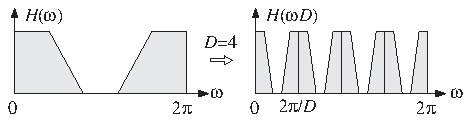
\includegraphics[width = 0.45\textwidth]{pic/combNotchStauchung.pdf}\\[-1.4cm]
	\end{itemize}
	\subsection{Notch-Filter}
		\vspace*{-0.3cm}\begin{minipage}{0.625\textwidth}
			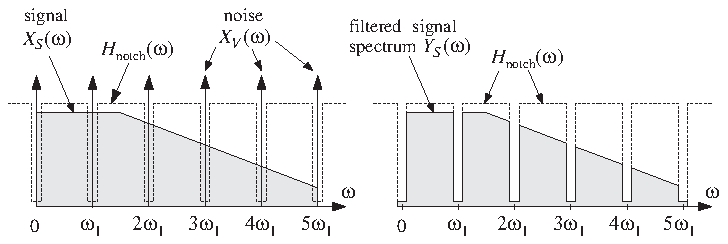
\includegraphics[width = \textwidth]{pic/notchFilter.pdf}\\[1.9cm]
		\end{minipage}\begin{minipage}[t]{0.075\textwidth}$ $\end{minipage}
		\begin{minipage}{0.3\textwidth}
			$\qquad$\begin{tikzpicture}[>=latex, scale=1.6]
				\def\s{2.7};
				\def\f{1.15};
				\def\r{0.9};
				\def\roc{0.9};
				\def\n{11};
				\coordinate (c1) at (0,0);
				\draw[line width=0.5](c1)++(-\s/2,-\s/2)--node[above,yshift=-1pt,xshift=-8pt]{\footnotesize$k=0,1,2,...,D-1$}++(\s,0)--++(0,\s)node[below left]{\small$z$-Plane}--++(-\s,0)--cycle node[below right, CadetRed]{\textbf{ }};
				\draw[line width=0.75](c1)--++(-\f,0)--++(2*\f,0)--++(-\f,0)--++(0,-\f)--++(0,2*\f)--++(0,-\f)circle(0);
				\draw[line width=0.5,dashed](c1)circle(\roc);
				\draw[line width=0.5,dashed](c1)circle(0.7);
				\draw[line width=0.75](c1)++(\roc,0.1)--++(0,-0.2)node[below right=-1pt,yshift=2pt]{$1$};
				\draw[line width=0.75](c1)++(-\roc,0.1)--++(0,-0.2)node[below left=-1pt,yshift=2pt]{-$1$};
				\draw[line width=0.75](c1)++(0.7,0.1)--++(0,-0.2);


				\draw[line width=2,white](c1)++(\s/2,0)++(0,0.05)--++(0,0.5);

				\draw[line width=0.75,dotted](c1)--++({360*0/\n}:1.2);
				\draw[line width=0.75,->](c1)++({360*0/\n}:1.1)arc({360*0/\n}:{360*1/\n}:1.1)node[below right, xshift=5pt,yshift=0pt]{\Large$\frac{2\pi k}{D}$};
				\draw[line width=0.75,dotted](c1)--++({360*1/\n}:1.2);



				
				\foreach \i in {0,1,2,...,10}
				{
					\draw[line width=0.75,dotted](c1)--++({360*\i/\n}:1);
					\draw[CadetRed,line width=0.75,fill=white](c1)++({360*\i/\n}:0.9)circle(\r/15);
					\draw[line width=0.75,fill,CadetRed](c1)++({360*\i/\n}:0.7)circle(\r/15);
				}

				\draw[line width=1,white](c1)++({360*10/\n}:0.3)--++({360*10/\n}:0.3);

				\draw[line width=0.75](c1)++(0.7,0.1)node[black,below left,yshift=-2pt]{$\sqrt[n]{a}$};

			\end{tikzpicture}
		\end{minipage}\\[-2.15cm]
		\begin{tabular}{ll}
			$3\,\db$-Bandbreite $\Delta\omega$: & \fcolorbox{CadetRed}{white}{$\beta = \tan\left(\dfrac{D\Delta\omega}{4}\right),\qquad a=\dfrac{1-\beta}{1+\beta},\qquad b = \dfrac{1}{1+\beta}$}\\[0.5cm]
			&$\begin{array}{l}0\leq a<1\\0<\beta\leq 1\end{array}\quad\Rightarrow\quad\Delta\omega \leq\dfrac{\pi}{D}\quad\Rightarrow\quad \Delta f\leq\dfrac{f_s}{2D}$\\[0.4cm]
			Übertragungsfunktion: &\fcolorbox{CadetRed}{white}{$H_{\text{notch}}(z) = b\dfrac{1-z^{-D}}{1-a\,z^{-D}}$}$\quad\;$\fcolorbox{CadetRed}{white}{$\big| H_{\text{notch}}(\omega)\big|^2 = \dfrac{\tan^2(\omega D/2)}{\tan^2(\omega D/2)+\beta^2}$}$\quad\;$ \fcolorbox{CadetRed}{white}{$NRR =b=\dfrac{1+a}{2}$}
		\end{tabular}

	\subsection{Comb-Filter}
		\vspace*{-0.3cm}\begin{minipage}{0.625\textwidth}
			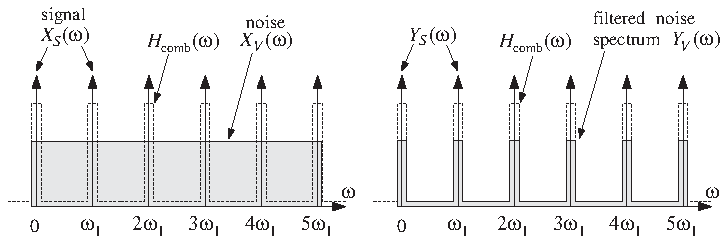
\includegraphics[width = \textwidth]{pic/combFilter.pdf}\\[1.9cm]
		\end{minipage}\begin{minipage}[t]{0.075\textwidth}$ $\end{minipage}
		\begin{minipage}{0.3\textwidth}
			$\qquad$\begin{tikzpicture}[>=latex, scale=1.6]
				\def\s{2.7};
				\def\f{1.15};
				\def\r{0.9};
				\def\roc{0.9};
				\def\n{11};
				\coordinate (c1) at (0,0);
				\draw[line width=0.5](c1)++(-\s/2,-\s/2)--node[above,yshift=-1pt,xshift=-8pt]{\footnotesize$k=0,1,2,...,D-1$}++(\s,0)--++(0,\s)node[below left]{\small$z$-Plane}--++(-\s,0)--cycle node[below right, CadetRed]{\textbf{ }};
				\draw[line width=0.75](c1)--++(-\f,0)--++(2*\f,0)--++(-\f,0)--++(0,-\f)--++(0,2*\f)--++(0,-\f)circle(0);
				\draw[line width=0.5,dashed](c1)circle(\roc);
				\draw[line width=0.5,dashed](c1)circle(0.7);
				\draw[line width=0.75](c1)++(\roc,0.1)--++(0,-0.2)node[below right=-1pt,yshift=2pt]{$1$};
				\draw[line width=0.75](c1)++(-\roc,0.1)--++(0,-0.2)node[below left=-1pt,yshift=2pt]{-$1$};
				\draw[line width=0.75](c1)++(0.7,0.1)--++(0,-0.2);


				\draw[line width=2,white](c1)++(\s/2,0)++(0,0.075)--++(0,0.45);
				\draw[line width=0.75,->](c1)++({360*0/\n}:1.15)node[above right, xshift=-3pt,yshift=1.5pt]{\Large$\frac{2\pi k}{D}$}arc({360*0/\n}:{360*1/\n}:1.1);
				\draw[line width=0.75,dotted](c1)--++({360*1/\n}:1.25);

				\draw[line width=2,white](c1)++(\s/2,0)++(0,-0.4)--++(0,-0.475);
				\draw[line width=0.75,->](c1)++({360*0/\n}:1.15)--++(0:0.05)--++(0:-0.05)node[below right, xshift=-10pt,yshift=-15pt]{\Large-$\frac{2\pi k+\pi}{D}$}arc({360*0/\n}:{-360*2/\n+180/\n}:1.1);
				\draw[line width=0.75,dotted](c1)--++({-360*2/\n+180/\n}:1.25);


				
				\foreach \i in {0,1,2,...,10}
				{
					\draw[line width=0.75,dotted](c1)--++({360*\i/\n}:1);
					\draw[CadetRed,line width=0.75,fill=white](c1)++({360*\i/\n+180/\n}:0.9)circle(\r/15);
					\draw[line width=0.75,fill,CadetRed](c1)++({360*\i/\n}:0.7)circle(\r/15);
				}

				\draw[line width=1,white](c1)++({360*10/\n}:0.3)--++({360*10/\n}:0.3);

				\draw[line width=0.75](c1)++(0.7,0.1)node[black,below left,yshift=-2pt]{$\sqrt[n]{a}$};

			\end{tikzpicture}
		\end{minipage}\\[-2.15cm]
		\begin{tabular}{ll}
			$3\,\db$-Bandbreite $\Delta\omega$: & \fcolorbox{CadetRed}{white}{$\beta = \tan\left(\dfrac{D\Delta\omega}{4}\right),\qquad a=\dfrac{1-\beta}{1+\beta},\qquad b = \dfrac{\beta}{1+\beta}$}\\[0.5cm]
			&$\begin{array}{l}0\leq a<1\\0<\beta\leq 1\end{array}\quad\Rightarrow\quad\Delta\omega \leq\dfrac{\pi}{D}\quad\Rightarrow\quad \Delta f\leq\dfrac{f_s}{2D}$\\[0.4cm]
			Übertragungsfunktion: &\fcolorbox{CadetRed}{white}{$H_{\text{comb}}(z) = b\dfrac{1+z^{-D}}{1-a\,z^{-D}}$}$\quad\;$\fcolorbox{CadetRed}{white}{$\big| H_{\text{comb}}(\omega)\big|^2 = \dfrac{\beta^2}{\tan^2(\omega D/2)+\beta^2}$}$\quad\;$ \fcolorbox{CadetRed}{white}{$NRR = b=\dfrac{1-a}{2}$}
		\end{tabular}
		
		\begin{info}
		 Die Noise-Reduction-Ratio bleibt gleich, wenn das Spektrum nur gestaucht wird. D.h. Die NNR der Notch- und Comb-Filter entspricht der NNR der entsprechenden Filter erster Ordnung.
		\end{info}

\newpage
\section{Signal-Mittelung }
	\begin{goal}
	 Von einem periodischen verrauschten Signal werden die Perioden gemittelt um das Rauschen zu unterdrücken. Diese Methode der Rauschunterdrückung resultiert in einem FIR-Comb-Filter und wird für die Verarbeitung von endlich langen Signal-Aufzeichnungen verwendet. 
	\end{goal}\\[-0.6cm]
	
	\begin{minipage}{0.6\textwidth}
		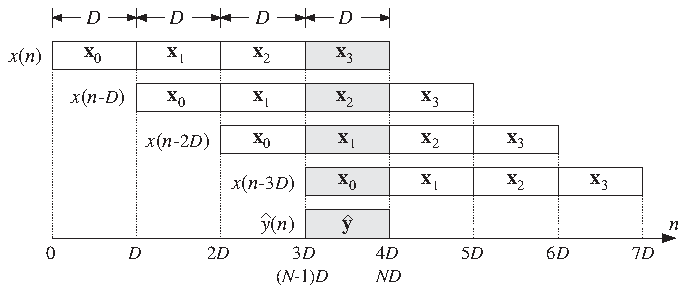
\includegraphics[width = \textwidth]{pic/signalAveraging1.pdf}
	\end{minipage}
	\begin{minipage}{0.4\textwidth}
		$\Rightarrow\quad$ \fcolorbox{CadetRed}{white}{$\begin{array}{l}\textbf{Mittelung über $\bm{N}$ Perioden}\\\textbf{mit der Länge $D$}\end{array}$}\\[0.4cm]
	\end{minipage}\\[0.2cm]
	\begin{tabular}{ll}
	 Gemitteltes Signal: & \fcolorbox{CadetRed}{white}{$\widehat{y}(n) = \dfrac{1}{N}\mysum{i=0}{N-1}{x(n-i\,D)}=\dfrac{1}{N}\mysum{i=0}{N-1}{x_i(n)} $}$\qquad n=0,1,2,...,D-1$\\[0.5cm]
	 Übertragungsfunktion: $\quad$& \fcolorbox{CadetRed}{white}{$H(z) = \dfrac{1}{N}(1+z^{-D}+z^{-2D}+...+z^{-(N-1)D}) = \dfrac{1}{N}\,\dfrac{1-z^{-ND}}{1-z^{-D}}$}\\[0.5cm]
	 Frequenzgang: & \fcolorbox{CadetRed}{white}{$H(\omega) = \dfrac{1}{N}\dfrac{\sin(ND\omega/2)}{\sin(D\omega/2)}$}$\qquad\quad$\fcolorbox{CadetRed}{white}{$\big|H(\omega)\big|^2 = \dfrac{1}{N^2}\dfrac{\sin^2(ND\omega/2)}{\sin^2(D\omega/2)}$}\\[0.5cm]
	 Grenzfrequenz: & \fcolorbox{CadetRed}{white}{$\omega_c = \dfrac{\pi}{ND}$}\\[0.5cm]
	 Noise-Reduction-Ratio:&\fcolorbox{CadetRed}{white}{$NRR = \dfrac{1}{N}$}
	\end{tabular}\\[0.2cm]
	
	\begin{info}
	 Dieses Filter erhält man auch, wenn man das Spektrum des FIR-Mittelungs-Filter $y(n) = [x(n)+x(n-1)+...+x(n-(N-1))]/N$ um den Faktor $D$ staucht ($z$ durch $z^D$ ersetzen)
	\end{info}
	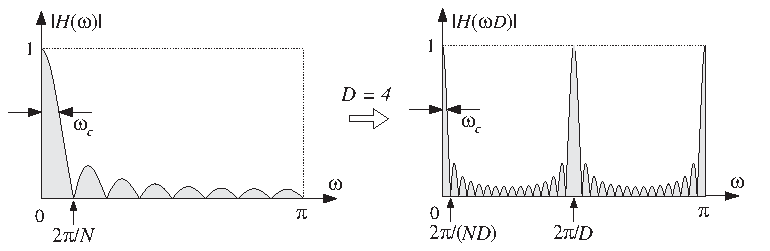
\includegraphics[width = 0.7\textwidth]{pic/signalAveraging.pdf}

	 Es resultiert ein Ausgangssignal das um den Faktor $1/N$ weniger stark rauscht.\\[0.2cm]
	 \fcolorbox{CadetRed}{white}{$\begin{array}{lcl}\widehat{y}(n)& =& y_S(n)+y_V(n)\\& = &x_S(n)+y_V(n)\end{array}$}$\qquad$
	 \fcolorbox{CadetRed}{white}{$\sigma_{Y_V}^2 = \dfrac{1}{N}\sigma_{X_V}^2$}\\

\newpage
\section{Savitzky-Golay-Smoothing-Filter}
	\begin{goal}
	 Die Idee ist, ein Polynom $p$-ter Ordnung optimal (Least-Square) in $N = 2M+1$ gemessene Samples einzupassen und anschliessend das mittlere Sample durch den Wert des Polynoms an dieser Stelle zu ersetzen. Dadurch wird das Rauschen reduziert. Zudem muss gelten $\quad$\fcolorbox{CadetRed}{white}{$N\geq p+1$}
	\end{goal}

	\textbf{Polynom-Beispiele mit N=5 Samples:}\\[0.2cm]
	\begin{tabularx}{\textwidth}{>{\centering\arraybackslash}X|>{\centering\arraybackslash}X|>{\centering\arraybackslash}X>{\centering\arraybackslash}X}
	 Konstante: & Linear: & Quadratisch: & \\[0.1cm]
	 \fcolorbox{CadetRed}{white}{$ \widehat{x}_m = c_0 $}&\fcolorbox{CadetRed}{white}{$\widehat{x}_m = c_0 + c_1\,m$}&\fcolorbox{CadetRed}{white}{$\widehat{x}_m = c_0 + c_1\,m+c_2\,m^2$}&\\
	 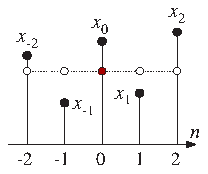
\includegraphics[width = 0.23\textwidth]{pic/SavitzkyGolayKonst.pdf} & 
	 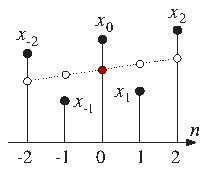
\includegraphics[width = 0.23\textwidth]{pic/SavitzkyGolayLin.pdf} & 
	 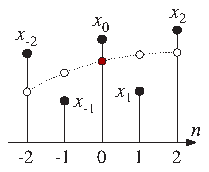
\includegraphics[width = 0.23\textwidth]{pic/SavitzkyGolayQuad.pdf} &
	 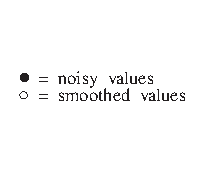
\includegraphics[width = 0.23\textwidth]{pic/SavitzkyGolayLeg.pdf}\\
	\end{tabularx}

	\subsection{Optimierungsproblem}
		Das Ziel ist ein Polynom $p$-ten Grades zu finden, welches den kleinsten quadratischen Fehler hat.\\[0.2cm]
		Minimiere:$\qquad$\fcolorbox{CadetRed}{white}{$\mathcal{J}\; = \mysum{m=-M}{M}{e_m^2}\;\; = \mysum{m=-M}{M}{(x_m - \widehat{x}_m)^2} = \mysum{m=-M}{M}{(x_m-(c_0 + c_1\,m + c_2\,m^2 + ... + c_p\,m^p))^2}$}\\[0.2cm]
		oder in Matrixschreibweise: $\qquad$\fcolorbox{CadetRed}{white}{$\mathcal{J} \;=\; \vec{e}\,^{\mathsf T}\vec e \;=\;(\vec x-S\,\vec c\,)^{\mathsf T}(\vec x-S\,\vec c\,) \;=\; \vec x\,^{\mathsf T}\vec x \;-\;2\,\vec c\,^{\mathsf T}S\,^{\mathsf T}\vec x\; +\; \vec c\,^{\mathsf T}S\,^{\mathsf T}S\,\vec c$}\\[0.2cm]
		\hspace*{2.6cm}mit $\qquad$ \fcolorbox{black}{white}{
		$\quad\vec c =\begin{bmatrix}c_0\\c_1\\c_2\\\vdots\\ c_p \end{bmatrix}$,
		$\qquad\vec x =\begin{bmatrix}x_{-M}\\\vdots\\x_{-1}\\x_0\\x_1\\\vdots\\ x_M \end{bmatrix}$,
		$\qquad\vec{ \widehat{x} }=\begin{bmatrix}\widehat x_{-M}\\\vdots\\\widehat x_{-1}\\\widehat x_0\\\widehat x_1\\\vdots\\ \widehat x_M \end{bmatrix} = S\,\vec c$,
		$\qquad \vec e = \vec x-\vec{\widehat x}\quad$}\\[0.2cm]
		\hspace*{2.6cm}und $\qquad\!$ \fcolorbox{black}{white}{
		$ \quad S = \begin{bmatrix}\vec s_0 & \vec s_1 &\vec s_2& \cdots &\vec s_p\end{bmatrix} = 
		\begin{bmatrix}	1 & -M & (-M)^2 & \cdots & (-M)^p\\[-0.15cm] 
				\vdots & \vdots & \vdots & \iddots & \vdots\\
				1 & -2& 4& \cdots& (-2)^p\\ 
				1 & -1& 1& \cdots& (-1)^p\\
				1 & 0& 0& \cdots& 0\\
				1 & 1& 1& \cdots& 1\\
				1 & 2& 4& \cdots& 2^p\\[-0.15cm] 
				\vdots & \vdots & \vdots & \ddots & \vdots\\
				1 & M& M^2& \cdots& M^p\\\end{bmatrix},\qquad \vec s_i(m) = m^i$}\\[0.2cm]
		Daraus folgt:$\qquad$\fcolorbox{CadetRed}{white}{$\dfrac{\partial \mathcal{J}}{\partial\vec c}\;=\; -\;2\,S\,^{\mathsf T}\vec x\; +\;2\, S\,^{\mathsf T}S\,\vec c\; \bm{=\; 0}$}$\qquad\Rightarrow\qquad$\fcolorbox{CadetRed}{white}{$\vec c = (S\,^{\mathsf T}S)^{-1}S\,^{\mathsf T}\vec x\;=\; G^{\mathsf T}\vec x$}\\[0.2cm]
		Die gefilterten Samples $\widehat x_m$ (Polynomwerte) können also folgendermassen berechnet werden:\\[0.2cm]
		\hspace*{0.3cm}$\Rightarrow\quad$\fcolorbox{CadetRed}{white}{$\vec{\widehat x}\;=\; S\,\vec c\;=\; S\,G^{\mathsf T}\vec x\; =\; S\,(S\,^{\mathsf T}S)^{-1}S\,^{\mathsf T}\vec x\;=\; B\,\vec x$}\\[0.2cm]
		\hspace*{1.1cm}mit$\qquad$\fcolorbox{black}{white}{$B = B\,^{\mathsf T} = S\,G\,^{\mathsf T} = S\,(S\,^{\mathsf T}S)^{-1}S\,^{\mathsf T} = S\,F^{-1}S\,^{\mathsf T} = \begin{bmatrix}\vec b_{-M} &\cdots&\vec b_{-1} &\vec b_0 &\vec b_1 &\cdots&\vec b_M \end{bmatrix}$}\\[0.2cm]
		\hspace*{1.1cm}und$\qquad\!$\fcolorbox{black}{white}{$G = S\,(S\,^{\mathsf T}S)^{-1} = S\,F^{-1} = \begin{bmatrix}\vec g_0 &\vec g_1 &\vec g_2 &\cdots&\vec g_p \end{bmatrix}$}$\qquad$
		und$\qquad\!$\fcolorbox{black}{white}{$F = S\,^{\mathsf T}S$}
\newpage
		
	\subsection{Matrizen für $\bm{M=2}$ und $\bm{p=2}$}
		\begin{tabularx}{\textwidth}{>{\centering\arraybackslash}X|>{\centering\arraybackslash}X|>{\centering\arraybackslash}X}
		 Matrix $S$: & Matrix $F$: & Inverse Matrix $F$:\\[0.2cm]
		 $S = \begin{bmatrix}1 & -2& 4\\1 & -1& 1\\1 & 0& 0\\1 & 1& 1\\1 & 2& 4\end{bmatrix}$&
		 $F = S\,^{\mathsf T}S \begin{bmatrix}5 & 0 & 10\\ 0 & 10 & 0\\ 10 &0 & 34\end{bmatrix}$&$F^{-1} =\dfrac{1}{35} \begin{bmatrix}17 & 0 & -5\\ 0 & 3.5 & 0\\ -5 &0 & 2.5\end{bmatrix}$\\[1.2cm]
		 \hline
		\end{tabularx}
		\begin{tabularx}{\textwidth}{>{\centering\arraybackslash}X|>{\centering\arraybackslash}X}
		 &\\[-0.2cm]
		 Matrix $G$: & Matrix $B$: \\[0.2cm]
		 $G = S\,F^{-1} = \dfrac{1}{35}\begin{bmatrix}-3 & -7 & 5\\ 12 & -3.5 & -2.5 \\ 17 & 0 & -5 \\12 & 3.5 & -2.5 \\ -3 & 7 & 5\end{bmatrix}$
		 & $B = S\,G\,^{\mathsf T} =\dfrac{1}{35}\begin{bmatrix} 31 & 9 & -3 & -5 & 3 \\ 9 & 13 & 12 & 6 & -5 \\ -3 & 12 & 17 & 12 & -3 \\ -5 & 6 & 12 & 13 & 9 \\ 3 & -5 & -3 & 9 & 31 \end{bmatrix}$\\[1.1cm]
		 $\qquad\qquad = \begin{bmatrix}\vec g_0 &\vec g_1 &\vec g_2 \end{bmatrix}$ & $\qquad\qquad\;\;\;\;\; = \begin{bmatrix}\vec b_{-2} &\vec b_{-1} &\vec b_0 &\vec b_1 &\vec b_2 \end{bmatrix}$\\[0.3cm]
		 \hline
		\end{tabularx}\\[0.2cm]

	\subsection{FIR-Smoothing-Filter}
		\begin{itemize}
		 \item Die gefilterten Samples $\widehat x_m$ (Polynomwerte) können nun folgendermassen berechnet werden:\\[0.2cm]
		 \fcolorbox{CadetRed}{white}{$\vec{\widehat{x}} = B\,\vec x  = B\,^{\mathsf T}\vec x =\begin{bmatrix}\vec b_{-M}^{\,\,\mathsf T}\vec x \\\vdots\\\vec b_{-1}^{\,\,\mathsf T}\vec x \\\vec b_0^{\,\,\mathsf T}\vec x \\\vec b_1^{\,\,\mathsf T}\vec x \\\vdots\\\vec b_M^{\,\,\mathsf T}\vec x\end{bmatrix}$}$\qquad\qquad$
		 $\begin{array}{l}\text{Oder wenn nur ein bestimmtes Sample,}\\\text{meistens das mittlere $(m=0)$, von Interesse ist:}\\[0.2cm]\text{\fcolorbox{CadetRed}{white}{$\widehat{x}_m = b_m^{\,\mathsf T}\,\vec x$}$\quad m = -M,...,-2,-1,0,1,2,...,M$}\end{array}$\\[-0.1cm]
		 \item Die Polynom-Koeffizienten können ebenfalls folgendermassen berechnet werden:\\[0.2cm]
		 \fcolorbox{CadetRed}{white}{$\vec c = G\,^{\mathsf T}\vec x =\begin{bmatrix}\vec g_0^{\,\,\mathsf T}\vec x \\\vec g_1^{\,\,\mathsf T}\vec x \\\vec g_2^{\,\,\mathsf T}\vec x\\\vdots\\\vec g_p^{\,\,\mathsf T}\vec x\end{bmatrix}$}$\qquad\qquad$\fcolorbox{CadetRed}{white}{${c}_i = g_i^{\,\mathsf T}\vec x$}$\quad i = 0,1,2,...,p$\\[-0.1cm]
		 \item Das Savitzky-Golay-Smoothing-Filter (für das mittlere Sample) kann also folgendermassen als FIR-Filter implementiert werden:\\[0.2cm]
		 \fcolorbox{CadetRed}{white}{$y_0 = \widehat{x}_0 = c_0 = b_0^{\,\,\mathsf T}\vec x = g_0^{\,\,\mathsf T}\vec x = \mysum{m=-M}{M}{b_0(m)\,x_m}$}\\[0.3cm]
		 Oder konkret für $M=2$ und $p=2$:\\[0.2cm]
		 \fcolorbox{CadetRed}{white}{$y(n) = \dfrac{-3\,x(n-2) + 12 \,x(n-1) + 17\,x(n)+ 12\, x(n+1) -3\,x(n+2)}{35}$}\\[-0.15cm]
		 \item Das resultierende FIR Filter hat einen DC-Gain von $1$ und keine Phase. Durch eine Verzögerung von $M$ Samples wird es kausal und linearphasig.\\[-0.45cm]
		 \item Das FIR-Filter hat eine Noise-Reduction-Ratio von:\\[0.2cm]
		 \fcolorbox{CadetRed}{white}{$NRR = \vec b_0^{\,\,\mathsf T}\vec b_0 = \mysum{m=-M}{M}{b_0(m)^2}  = b_0(0) = \dfrac{17}{35} = 0.49$}
		\end{itemize}

\newpage
	\subsection{Ableiten und integrieren mit Savitzky-Golay-Smoothing-Filter}
		Das das Savitzky-Golay-Smoothing-Filter ein Polynom in die gemessenen Samples hineinpasst ist es sehr gut geeignet, um das Signal mittels dieses Polynoms abzuleiten oder zu integrieren\\[0.3cm]
		\textbf{Ableiten mit Savitzky-Golay-Smoothing-Filter:}\\[0.2cm]
		\begin{tabularx}{\textwidth}{cX}
		 \multicolumn{2}{l}{Polynom:} \\[0.1cm]
		 &\fcolorbox{black}{white}{$y_m = \widehat x_m = c_0 + c_1\,m + c_2\,m^2 + ... + c_p\,m^p$}\\[0.4cm]
		 \multicolumn{2}{l}{erste Ableitung:}\\[0.1cm]
		 & $\dot {y}_m = c_1 + 2\,c_2\,m + 3\,c_3\,m^2 + ... + p\,c_p\,m^{p-1}\qquad\Rightarrow\qquad m=0\qquad\Rightarrow\qquad $\fcolorbox{CadetRed}{white}{$\dot {y}_0 = c_1 = g_1^{\,\mathsf T}\vec x$}\\[0.3cm]
		 \multicolumn{2}{l}{zweite Ableitung:}\\[0.1cm]
		 &$\ddot {y}_m = 2\,c_2 + 6\,c_3\,m + ... + p\,(p-1)\,c_p\,m^{p-2}\qquad\Rightarrow\qquad m=0\qquad\Rightarrow\qquad $\fcolorbox{CadetRed}{white}{$\ddot {y}_0 = 2\,c_2 = 2\,g_2^{\,\mathsf T}\vec x$}\\[0.3cm]
		 \multicolumn{2}{l}{$i$-te Ableitung:}\\[0.1cm]
		 &${y}_m^{(i)} = i!\,c_i + (i-1)!\,c_{i-1}\,m + ... + $\text{\small$\dfrac{p!}{(p-i-1)!}$}$\,c_p\,m^{p-i}\qquad\Rightarrow\qquad m=0\qquad\Rightarrow\qquad $\fcolorbox{CadetRed}{white}{${y}_0^{(i)} = i!\,c_i = i!\,g_i^{\,\mathsf T}\vec x$}\\[0.4cm]
		 &\\[-0.3cm]
		 \multicolumn{2}{l}{\textbf{Ableitung für $\bm{M=2}$ und $\bm{p=2}$}} \\[0.1cm]
		 &\\[-0.3cm]
		 \multicolumn{2}{l}{\fcolorbox{CadetRed}{white}{$\dot{y}_n = \dfrac{1}{35}\,\big(-7\,x_{n-2}-3.5\,x_{n-1}+3.5\,x_{n+1}+7\,x_{n+2}\big)$}$\quad$\fcolorbox{CadetRed}{white}{$\ddot{y}_n = \dfrac{2}{35}\,\big(5\,x_{n-2}-2.5\,x_{n-1}-5\,x_n-2.5\,x_{n+1}+5\,x_{n+2}\big)$}}\\[0.4cm]	 
		\end{tabularx}\\[0.1cm]
		
		\textbf{Integrieren mit Savitzky-Golay-Smoothing-Filter:}\\[0.2cm]
		\begin{tabularx}{\textwidth}{cX}
		 \multicolumn{2}{l}{Polynom:} \\[0.1cm]
		 &\fcolorbox{black}{white}{$y_m = \widehat x_m = c_0 + c_1\,m + c_2\,m^2 + ... + c_p\,m^p$}\\[0.4cm]
		 \multicolumn{2}{l}{ein Integral-Intervall:}\\[0.1cm]
		 & $\begin{array}{lcl}i[n]& = &\myint{-1/2}{1/2}{\widehat{x}_m}{m}\; =\; \myint{-1/2}{1/2}{c_0 + c_1\,m + c_2\,m^2 + ... + c_p\,m^p}{m}\\& =& \left[c_o\,m + \dfrac{c_1}{2}m^2 + \dfrac{c_2}{3}m^3+\dots+\dfrac{c_p}{p+1}m^{p+1}\right]_{-1/2}^{1/2}\\
		 & =&
		 \text{\small$\begin{cases}\\[-0.3cm]\begin{bmatrix}1 & 0 & \dfrac{1}{3\cdot2^2} & 0 & \dfrac{1}{5\cdot2^4} & \dots & 0 & \dfrac{1}{(p+1)\cdot2^p}\end{bmatrix}\cdot\vec c,& \text{$p$ ungerade}\\[0.3cm] \begin{bmatrix}1 & 0 & \dfrac{1}{3\cdot2^2} & 0 & \dfrac{1}{5\cdot2^4} & \dots& \dfrac{1}{p\cdot2^{p-1}} & 0\end{bmatrix}\cdot\vec c,& \text{$p$ gerade}\\[0.4cm]\end{cases}$}\\
		  & =&
		 \underline{\underline{\text{\small$\begin{cases}\\[-0.3cm]\begin{bmatrix}1 & 0 & \dfrac{1}{3\cdot2^2} & 0 & \dfrac{1}{5\cdot2^4} & \dots & 0 & \dfrac{1}{(p+1)\cdot2^p}\end{bmatrix}\cdot G\,^{\mathsf T}\vec x,& \text{$p$ ungerade}\\[0.3cm] \begin{bmatrix}1 & 0 & \dfrac{1}{3\cdot2^2} & 0 & \dfrac{1}{5\cdot2^4} & \dots& \dfrac{1}{p\cdot2^{p-1}} & 0\end{bmatrix}\cdot G\,^{\mathsf T}\vec x,& \text{$p$ gerade}\\[0.4cm]\end{cases}$}}}\end{array} $\\[3.6cm]
		 \multicolumn{2}{l}{alle Integral-Intervalle aufsummiert:}\\[0.2cm]
		 &\fcolorbox{CadetRed}{white}{$I[n] \;= \; \mysum{k=0}{n}{T\cdot i[k]} \;= \; \mysum{k=0}{n-1}{T\cdot i[k]} + T\cdot i[n] \;= \;I[n-1] + T\cdot i[n] $}\\[0.3cm]
		\end{tabularx}
